\PassOptionsToPackage{unicode=true}{hyperref} % options for packages loaded elsewhere
\PassOptionsToPackage{hyphens}{url}
%
\documentclass[12pt,ignorenonframetext,]{beamer}
\usepackage{pgfpages}
\setbeamertemplate{caption}[numbered]
\setbeamertemplate{caption label separator}{: }
\setbeamercolor{caption name}{fg=normal text.fg}
\beamertemplatenavigationsymbolsempty
% Prevent slide breaks in the middle of a paragraph:
\widowpenalties 1 10000
\raggedbottom
\setbeamertemplate{part page}{
\centering
\begin{beamercolorbox}[sep=16pt,center]{part title}
  \usebeamerfont{part title}\insertpart\par
\end{beamercolorbox}
}
\setbeamertemplate{section page}{
\centering
\begin{beamercolorbox}[sep=12pt,center]{part title}
  \usebeamerfont{section title}\insertsection\par
\end{beamercolorbox}
}
\setbeamertemplate{subsection page}{
\centering
\begin{beamercolorbox}[sep=8pt,center]{part title}
  \usebeamerfont{subsection title}\insertsubsection\par
\end{beamercolorbox}
}
\AtBeginPart{
  \frame{\partpage}
}
\AtBeginSection{
  \ifbibliography
  \else
    \frame{\sectionpage}
  \fi
}
\AtBeginSubsection{
  \frame{\subsectionpage}
}
\usepackage{lmodern}
\usepackage{amssymb,amsmath}
\usepackage{ifxetex,ifluatex}
\usepackage{fixltx2e} % provides \textsubscript
\ifnum 0\ifxetex 1\fi\ifluatex 1\fi=0 % if pdftex
  \usepackage[T1]{fontenc}
  \usepackage[utf8]{inputenc}
  \usepackage{textcomp} % provides euro and other symbols
\else % if luatex or xelatex
  \usepackage{unicode-math}
  \defaultfontfeatures{Ligatures=TeX,Scale=MatchLowercase}
\fi
\usetheme[]{Frankfurt}
\usecolortheme{lily}
% use upquote if available, for straight quotes in verbatim environments
\IfFileExists{upquote.sty}{\usepackage{upquote}}{}
% use microtype if available
\IfFileExists{microtype.sty}{%
\usepackage[]{microtype}
\UseMicrotypeSet[protrusion]{basicmath} % disable protrusion for tt fonts
}{}
\IfFileExists{parskip.sty}{%
\usepackage{parskip}
}{% else
\setlength{\parindent}{0pt}
\setlength{\parskip}{6pt plus 2pt minus 1pt}
}
\usepackage{hyperref}
\hypersetup{
            pdftitle={Strategic Decision Making in the 3D Printing Industry},
            pdfauthor={Pedro Nascimento de Lima; Maria I. W. M. Morandi; Daniel Pacheco Lacerda},
            pdfborder={0 0 0},
            breaklinks=true}
\urlstyle{same}  % don't use monospace font for urls
\newif\ifbibliography
\usepackage{longtable,booktabs}
\usepackage{caption}
% These lines are needed to make table captions work with longtable:
\makeatletter
\def\fnum@table{\tablename~\thetable}
\makeatother
\usepackage{graphicx,grffile}
\makeatletter
\def\maxwidth{\ifdim\Gin@nat@width>\linewidth\linewidth\else\Gin@nat@width\fi}
\def\maxheight{\ifdim\Gin@nat@height>\textheight\textheight\else\Gin@nat@height\fi}
\makeatother
% Scale images if necessary, so that they will not overflow the page
% margins by default, and it is still possible to overwrite the defaults
% using explicit options in \includegraphics[width, height, ...]{}
\setkeys{Gin}{width=\maxwidth,height=\maxheight,keepaspectratio}
\setlength{\emergencystretch}{3em}  % prevent overfull lines
\providecommand{\tightlist}{%
  \setlength{\itemsep}{0pt}\setlength{\parskip}{0pt}}
\setcounter{secnumdepth}{0}

% set default figure placement to htbp
\makeatletter
\def\fps@figure{htbp}
\makeatother

\def\begincols{\begin{columns}}
\def\begincol{\begin{column}}
\def\endcol{\end{column}}
\def\endcols{\end{columns}}

%\usepackage{fancyhdr}
%\pagestyle{fancy}
%\fancyhead[CO,CE]{This is fancy header}
%\fancyfoot[CO,CE]{And this is a fancy footer}
%\fancyfoot[LE,RO]{\thepage}


%\usepackage {hyperref}
%\hypersetup {colorlinks = true, linkcolor = blue, urlcolor = blue, citecolor = blue}


\setbeamertemplate{footline}[text line]{%
  \parbox{\linewidth}{\vspace*{-8pt}2018 DMDU Meeting\hfill\insertshortauthor\hfill\insertpagenumber}}

\setbeamertemplate{navigation symbols}{}

\title{Strategic Decision Making in the 3D Printing Industry}
\providecommand{\subtitle}[1]{}
\subtitle{A Robust Decision Making (RDM) analysis}
\author{Pedro Nascimento de Lima \and Maria I. W. M. Morandi \and Daniel Pacheco Lacerda}
\providecommand{\institute}[1]{}
\institute{GMAP Research Group, UNISINOS University, RS, Brazil \and 2018 DMDU Annual Meeting}
\date{November 14, 2018}

\begin{document}
\frame{\titlepage}

\hypertarget{introduction}{%
\section{Introduction}\label{introduction}}

\begin{frame}{Motivation - DMDU and Business Decisions}
\protect\hypertarget{motivation---dmdu-and-business-decisions}{}

\begin{itemize}
\tightlist
\item
  Decision Makers in Business are faced with uncertainty, but\ldots{}
\item
  Testing quotation: (Lima 2018), (Gong et al. 2017), (Wholers 2016).
\end{itemize}

\end{frame}

\begin{frame}{Key Features of 3D printing}
\protect\hypertarget{key-features-of-3d-printing}{}

\begin{itemize}
\tightlist
\item
  3D printing allows us to manufacture parts with unprecedented
  \textbf{complexity}, in \textbf{low volume};
\item
  By doing so, entire manufacturing industries might be disrupted by AM,
  presenting challenges to \ldots{}
\end{itemize}

\end{frame}

\begin{frame}{Two Column Layout}
\protect\hypertarget{two-column-layout}{}

\begincols
  \begincol{.48\textwidth}

\begin{itemize}
\item
  3D printing allows us to manufacture parts with unprecedented
  \textbf{complexity}, in \textbf{low volume};
\item
  By doing so, entire manufacturing industries might be disrupted by AM,
  presenting challenges to \ldots{}

  \endcol
  \begincol{.48\textwidth}
\end{itemize}

\includegraphics{dmdu-presentation_files/figure-beamer/test-1.pdf}

\endcol \endcols

\end{frame}

\begin{frame}{Why 3D Printing?}
\protect\hypertarget{why-3d-printing}{}

3D Printing is an emergint technology, but decision makers face
uncertainty:

\begincols
  \begincol{.48\textwidth}

\textbf{Positive Evidence}:

\begin{itemize}
\item
  3D printing Industry has seen two digits growth consistently in the
  last few years;
\item
  3D printing is already reshaping supply chains across industries
  (e.g.: prothesis, aerospace, etc.).

  \endcol
  \begincol{.48\textwidth}
\end{itemize}

\textbf{Negative Evidence}:

\begin{itemize}
\item
  Major players have been observing declining profitability (e.g.:
  Stratasys, 3D Systems);
\item
  Estimates of 3D printing growth diverge.

  \endcol
  \endcols
\end{itemize}

\end{frame}

\begin{frame}{Shaping Events and Factors in the 3D Printing Industry}
\protect\hypertarget{shaping-events-and-factors-in-the-3d-printing-industry}{}

\begin{itemize}
\tightlist
\item
  Patent Dynamics \& Patent Expiration: (e.g.~FDM Patent);
\item
  R \& D
\item
  Strong Competition:
\item
  After the 3D printing Bubble, major players refocused their operations
  on industrial-grade printers;
\end{itemize}

\end{frame}

\hypertarget{problem-structuring-xlrm}{%
\section{Problem Structuring / XLRM}\label{problem-structuring-xlrm}}

\begin{frame}{New Product Diffusion Models}
\protect\hypertarget{new-product-diffusion-models}{}

There is a broad range of models portraying new product diffusion and
technological substititions, beyond the basic Bass Diffusion Model (Bass
1969):

\begin{itemize}
\tightlist
\item
  New Product Launch Strategy and timing between successive Product
  Generations (Mahajan and Muller 1996);
\item
  Social Factors (e.g.~Reference Users and Opinion Leaders - GE in the
  case of AM) (Dattée and Birdseye Weil 2007);
\item
  Competition Among Players and Substitution Between Product Generations
  (Maier 1998);
\item
  Market Uncertainty (Cui, Zhao, and Ravichandran 2011);
\item
  Competition, Learning Curves, diffusion dynamics, Pricing and Capacity
  Strategies (Sterman et al. 2007).
\end{itemize}

\end{frame}

\begin{frame}{What's the Problem}
\protect\hypertarget{whats-the-problem}{}

\begin{itemize}
\item
  Most of these models are employed with a \textbf{consolidative}
  approach (model parameters are estimated from past products);
\item
  Some of them employ Senstitivity Analysis to explain under which
  conditions one might choose a different strategy based on thresholds
  of uncertain parameters.
\end{itemize}

\end{frame}

\begin{frame}{Sterman et. al (2007) Model}
\protect\hypertarget{sterman-et.-al-2007-model}{}

We have choosen (Sterman et al. 2007) model as a bed-rock for our
analysis, since :

\begin{itemize}
\tightlist
\item
  It Captures competition among players;
\item
  It Captures increasing returns mechanisms (Learning Curve);
\item
  It was fully documented, and provided the original model for
  comparisons, and;
\item
  Our goal was not to \textbf{focus on model development} but to focus
  on employing an \textbf{exploratory modelling} approach to the 3D
  printing industry.
\end{itemize}

\end{frame}

\begin{frame}{X - Uncertainties}
\protect\hypertarget{x---uncertainties}{}

\begin{itemize}
\item
  Market size and diffusion velocity is still unknown, reflecting on
  diverging industry forecasts;
\item
  Share prices of lead players have fallen between 71 \% and 80 \% in 17
  months in 2017 (Kelleher 2015);
\item
  Signals of Uncertainty for some, or Information Assimetry:
\item
  Major AM Systems Manufacturers have seen falling Net profits;
\end{itemize}

\end{frame}

\begin{frame}{X - Uncertainties}
\protect\hypertarget{x---uncertainties-1}{}

\begin{itemize}
\item
  Successfull 3D printing adoption for manufacturing final parts depends
  on changing \textbf{product engineering processess} towards a
  \textbf{design for AM} posture. (Aston 2017)
\item
  What the final market will prefer? A cheap, low-resolution printer or
  a high-quality, high-cost printer?
\item
  What if your competitor is able to provide a high-quality, low-cost
  printer?
\item
  How much capacity will your oponents build?
\end{itemize}

\end{frame}

\begin{frame}{L - Levers}
\protect\hypertarget{l---levers}{}

From (Sterman et al. 2007):

\begin{itemize}
\tightlist
\item
  \textbf{Pricing and Capacity Strategy}:
\item
  \textbf{Agressive}: Build capacity towards a target-market share;
  dynamicaly adjust your prices to leverage increasing returns (maybe at
  the expense of near term results);
\item
  \textbf{Conservative}: Define a minimum target market share, and
  adjust your pricing towards this share. Don't build excess capacity.
\end{itemize}

\end{frame}

\begin{frame}{L - Levers}
\protect\hypertarget{l---levers-1}{}

Relevant factors from the AM industry: - R \& D and printer performance
are key factor: - Patents are used by leading companies to deter new
entrants;

\end{frame}

\begin{frame}{R - Relationships}
\protect\hypertarget{r---relationships}{}

\end{frame}

\begin{frame}{M - Metrics}
\protect\hypertarget{m---metrics}{}

\end{frame}

\begin{frame}{Model Boundaries}
\protect\hypertarget{model-boundaries}{}

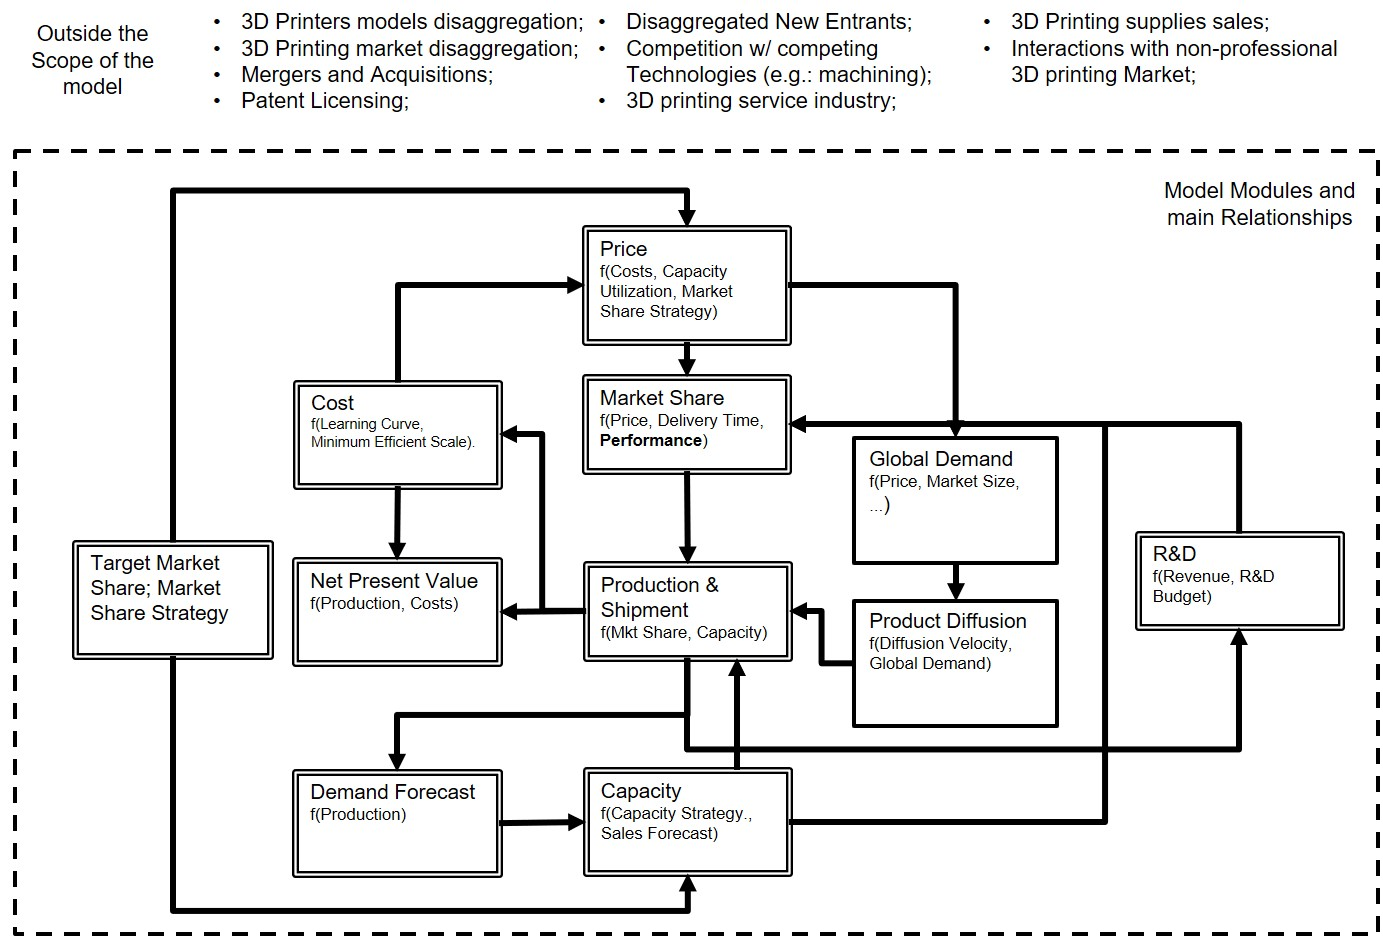
\includegraphics{images/model-modules-and-boundaries.jpg}

\end{frame}

\hypertarget{case-generation}{%
\section{Case Generation}\label{case-generation}}

\begin{frame}{Design of Experiments}
\protect\hypertarget{design-of-experiments}{}

\begin{itemize}
\tightlist
\item
  Full factorial design of these variables, resulting in 54 strategies:
\end{itemize}

\begin{longtable}[]{@{}lll@{}}
\toprule
\begin{minipage}[b]{0.14\columnwidth}\raggedright
Variable\strut
\end{minipage} & \begin{minipage}[b]{0.48\columnwidth}\raggedright
Meaning\strut
\end{minipage} & \begin{minipage}[b]{0.30\columnwidth}\raggedright
Levels\strut
\end{minipage}\tabularnewline
\midrule
\endhead
\begin{minipage}[t]{0.14\columnwidth}\raggedright
\(S_1\)\strut
\end{minipage} & \begin{minipage}[t]{0.48\columnwidth}\raggedright
Market \& Pricing Strategy. Defines wether the player pursue an
agressive marketing strategy to gain market share (by cutting prices and
accepting excess capacity), or pursue a conservative strategy,\strut
\end{minipage} & \begin{minipage}[t]{0.30\columnwidth}\raggedright
Agressive (1); Conservative (2)\strut
\end{minipage}\tabularnewline
\begin{minipage}[t]{0.14\columnwidth}\raggedright
\(S_1^{max}\) or \(S_1^{min}\)\strut
\end{minipage} & \begin{minipage}[t]{0.48\columnwidth}\raggedright
Desired Market Share. For a Conservative Strategy, the player adopts the
\(S_1^{max}\), and for an Agressive Strategy, \(S_1^{min}\)\strut
\end{minipage} & \begin{minipage}[t]{0.30\columnwidth}\raggedright
20\%; 30\%; 40\%\strut
\end{minipage}\tabularnewline
\begin{minipage}[t]{0.14\columnwidth}\raggedright
\(\eta_1\)\strut
\end{minipage} & \begin{minipage}[t]{0.48\columnwidth}\raggedright
R \& D budget, as a fraction of revenue.\strut
\end{minipage} & \begin{minipage}[t]{0.30\columnwidth}\raggedright
5\%; 10\%; 15\%\strut
\end{minipage}\tabularnewline
\begin{minipage}[t]{0.14\columnwidth}\raggedright
\(\kappa_i\)\strut
\end{minipage} & \begin{minipage}[t]{0.48\columnwidth}\raggedright
Fraction of R \& D budget released to open source technologies.\strut
\end{minipage} & \begin{minipage}[t]{0.30\columnwidth}\raggedright
0 \%; 50 \%; 90 \%\strut
\end{minipage}\tabularnewline
\bottomrule
\end{longtable}

\end{frame}

\begin{frame}{Candidate Strategy NPV across scenarios}
\protect\hypertarget{candidate-strategy-npv-across-scenarios}{}

\begin{center}\includegraphics{dmdu-presentation_files/figure-beamer/unnamed-chunk-1-1} \end{center}

\end{frame}

\begin{frame}{Global Demand across scenarios}
\protect\hypertarget{global-demand-across-scenarios}{}

\begin{center}\includegraphics{dmdu-presentation_files/figure-beamer/unnamed-chunk-2-1} \end{center}

\end{frame}

\begin{frame}{4 Players Net Present Value in a given scenario}
\protect\hypertarget{players-net-present-value-in-a-given-scenario}{}

\begin{center}\includegraphics{dmdu-presentation_files/figure-beamer/unnamed-chunk-3-1} \end{center}

\end{frame}

\begin{frame}{Net Present Value across strategies and Scenarios}
\protect\hypertarget{net-present-value-across-strategies-and-scenarios}{}

\begin{center}\includegraphics{dmdu-presentation_files/figure-beamer/unnamed-chunk-4-1} \end{center}

\end{frame}

\begin{frame}{Regret across strategies and Scenarios}
\protect\hypertarget{regret-across-strategies-and-scenarios}{}

\begin{center}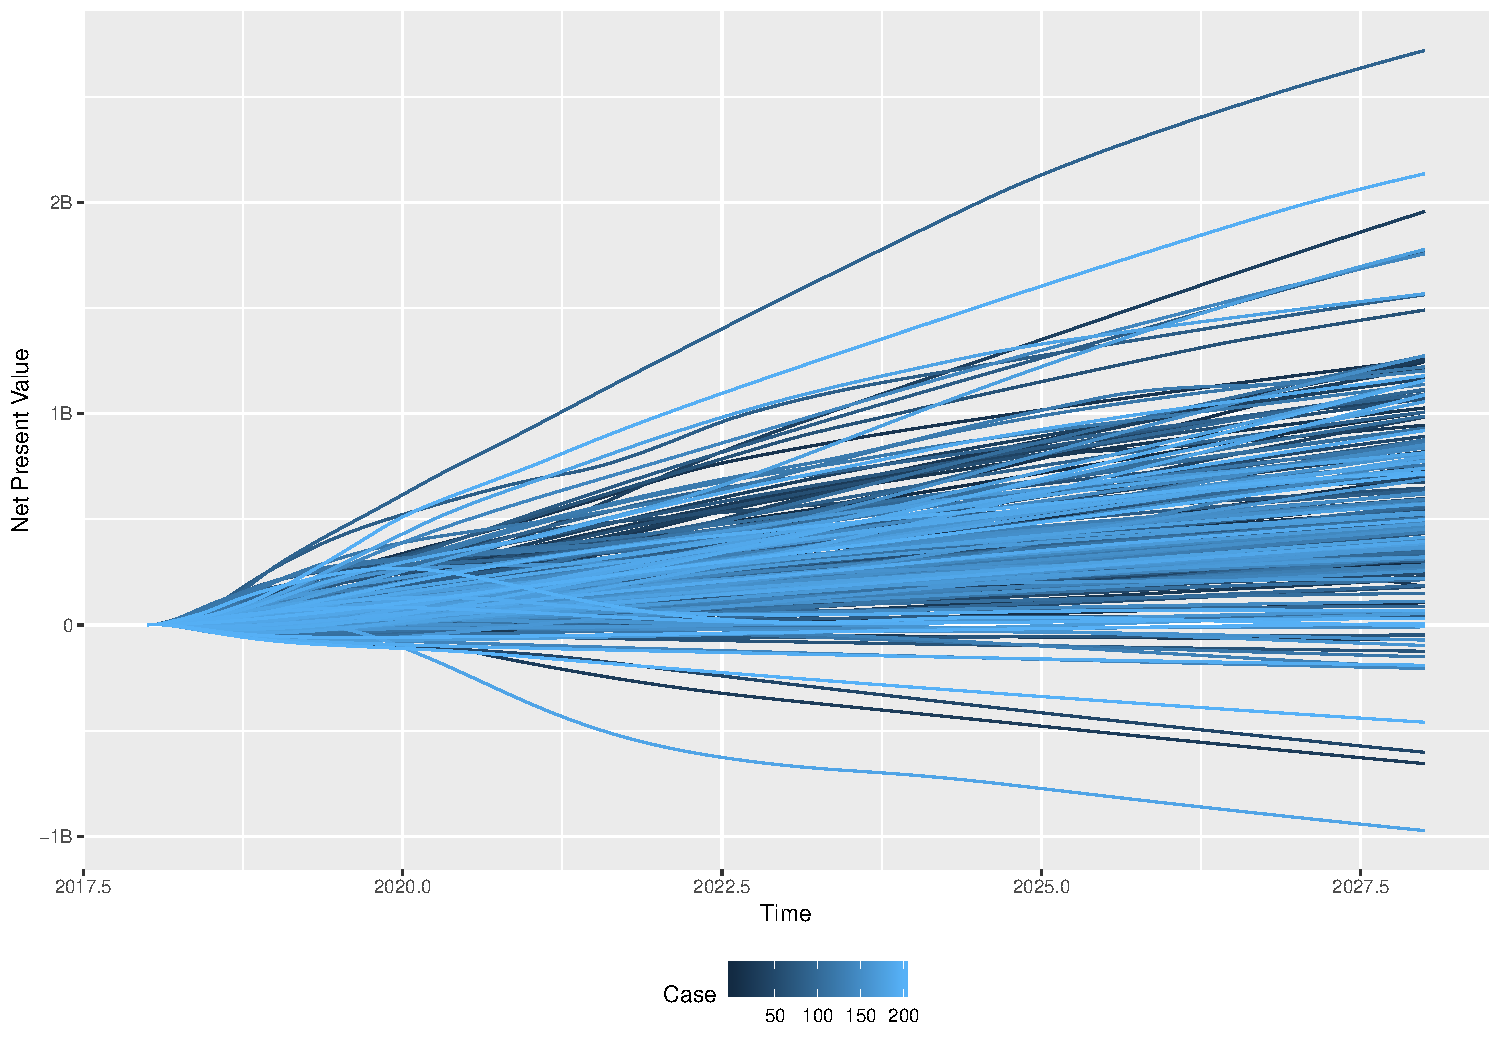
\includegraphics{dmdu-presentation_files/figure-beamer/unnamed-chunk-5-1} \end{center}

\end{frame}

\hypertarget{scenario-discovery}{%
\section{Scenario Discovery}\label{scenario-discovery}}

\hypertarget{conclusions}{%
\section{Conclusions}\label{conclusions}}

\begin{frame}{References}
\protect\hypertarget{references}{}

\hypertarget{refs}{}
\leavevmode\hypertarget{ref-Aston2017}{}%
Aston, Richard. 2017. ``3D Printing Done Right.''
\url{http://www.boeing.com/features/innovation-quarterly/nov2017/feature-thought-leadership-3d-printing.page}.

\leavevmode\hypertarget{ref-Bass1969}{}%
Bass, Frank M. 1969. ``A New Product Growth for Model Consumer
Durables.'' \emph{Management Science} 15 (5): 215--27.
\url{https://doi.org/10.1287/mnsc.15.5.215}.

\leavevmode\hypertarget{ref-Cui2011}{}%
Cui, Anna Shaojie, Meng Zhao, and T Ravichandran. 2011. ``Market
Uncertainty and Dynamic New Product Launch Strategies : A System
Dynamics Model.'' \emph{IEEE Transactions on Engineering Management} 58
(3): 530--50.

\leavevmode\hypertarget{ref-Dattee2007}{}%
Dattée, Brice, and Henry Birdseye Weil. 2007. ``Dynamics of social
factors in technological substitutions.'' \emph{Technological
Forecasting and Social Change} 74 (5): 579--607.
\url{https://doi.org/10.1016/j.techfore.2007.03.003}.

\leavevmode\hypertarget{ref-Gong2017}{}%
Gong, Min, Robert Lempert, Andrew Parker, Lauren A. Mayer, Jordan
Fischbach, Matthew Sisco, Zhimin Mao, David H. Krantz, and Howard
Kunreuther. 2017. ``Testing the scenario hypothesis: An experimental
comparison of scenarios and forecasts for decision support in a complex
decision environment.'' \emph{Environmental Modelling \& Software} 91.
Elsevier Ltd: 135--55.
\url{https://doi.org/10.1016/j.envsoft.2017.02.002}.

\leavevmode\hypertarget{ref-Kelleher2015}{}%
Kelleher, Kevin. 2015. ``Was 3D Printing Just a Passing Fad?''
\url{http://time.com/3916323/3d-printer-stocks/}.

\leavevmode\hypertarget{ref-Lima2018}{}%
Lima, Pedro Nascimento de. 2018. ``Avaliação de Decisões Estratégicas
sob Incerteza Profunda na Indústria da Manufatura Aditiva: Uma Análise a
partir do método Robust Decision Making (RDM).'' Masters Dissertation,
UNISINOS.
\url{http://www.repositorio.jesuita.org.br/handle/UNISINOS/6991}.

\leavevmode\hypertarget{ref-Mahajan1996}{}%
Mahajan, Vijay, and Eitan Muller. 1996. ``Timing, diffusion, and
substitution of successive generations of technological innovations: The
IBM mainframe case.'' \emph{Technological Forecasting and Social Change}
51 (2): 109--32. \url{https://doi.org/10.1016/0040-1625(95)00225-1}.

\leavevmode\hypertarget{ref-Maier1998}{}%
Maier, Frank H. 1998. ``New product diffusion models in innovation
management---a system dynamics perspective.'' \emph{System Dynamics
Review (Wiley)} 14 (4): 285--308.
\href{https://search.ebscohost.com/login.aspx?direct=true\%7B/\&\%7Ddb=bth\%7B/\&\%7DAN=17073696\%7B/\&\%7Dsite=ehost-live}{https://search.ebscohost.com/login.aspx?direct=true\{\textbackslash{}\&\}db=bth\{\textbackslash{}\&\}AN=17073696\{\textbackslash{}\&\}site=ehost-live}.

\leavevmode\hypertarget{ref-Sterman2007}{}%
Sterman, John D., Rebecca Henderson, Eric D. Beinhocker, and Lee I.
Newman. 2007. ``Getting Big Too Fast: Strategic Dynamics with Increasing
Returns and Bounded Rationality.'' \emph{Management Science} 53 (4):
683--96. \url{https://doi.org/10.1287/mnsc.1060.0673}.

\leavevmode\hypertarget{ref-Wholers2016}{}%
Wholers, Terry. 2016. ``Popularity of FDM.''
\url{https://wohlersassociates.com/blog/2016/01/popularity-of-fdm/}.

\end{frame}

\end{document}
